\section{Simulation Analysis}
\label{sec:simulation}

\subsection{Operating Point Analysis}

Table~\ref{tab:op} shows the simulated operating point results for the circuit under analysis.

\begin{table}[htb!]
  \centering
  \begin{tabular}{|l|r|}
    \hline    
    {\bf Name} & {\bf Value [A or V]} \\ \hline
    @gb[i] & -2.48284e-04\\ \hline
@r1[i] & 2.369027e-04\\ \hline
@r2[i] & -2.48284e-04\\ \hline
@r3[i] & -1.13810e-05\\ \hline
@r4[i] & 1.210640e-03\\ \hline
@r5[i] & -2.48284e-04\\ \hline
@r6[i] & 9.737374e-04\\ \hline
@r7[i] & 9.737374e-04\\ \hline
v(1) & 5.185042e+00\\ \hline
v(2) & 4.941554e+00\\ \hline
v(3) & 4.425830e+00\\ \hline
v(5) & 4.977013e+00\\ \hline
v(6) & 5.729012e+00\\ \hline
v(7) & -1.97652e+00\\ \hline
v(8) & -2.95469e+00\\ \hline
v(9) & 0.000000e+00\\ \hline

  \end{tabular}
  \caption{Operating point results. A variable preceded by @ is of type {\em current}
    and expressed in Ampere; other variables are of type {\it voltage} and expressed in
    Volt.}
  \label{tab:op}
\end{table}

These results were produced using the \textit{Ngspice software}. In order for the \textit{software} to be able to recognise the Current-Controlled Voltage Source, defined in Figure \ref{fig2} as $H_c$, we had to add a new Independent Voltage Source with a voltage of 0V, which is also represented in \ref{fig2}.


\begin{figure}[h] \centering
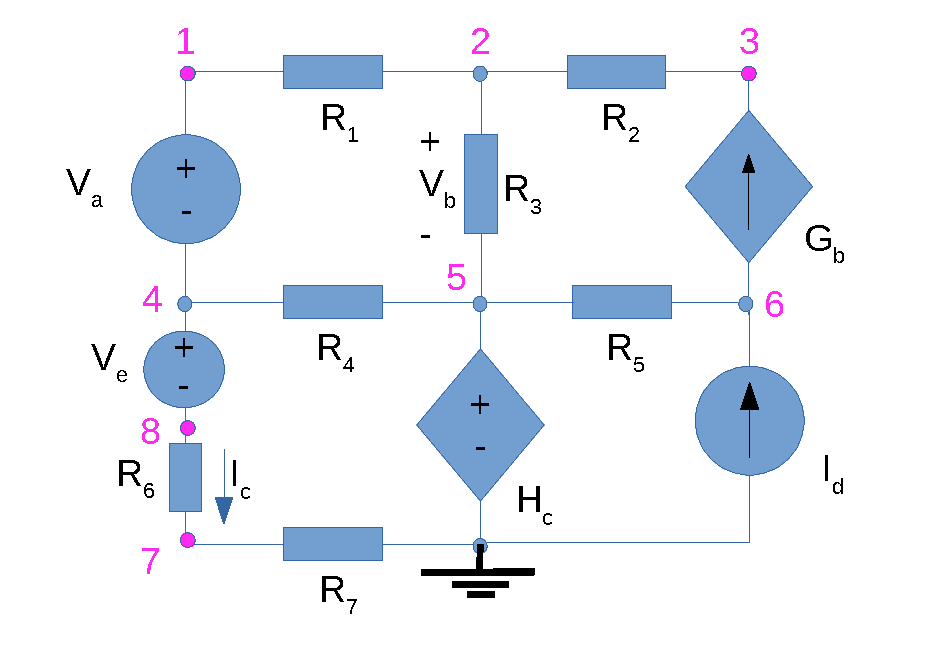
\includegraphics[width=0.4\linewidth]{t1-2.pdf}
\caption{The original circuit with an added voltage source of value 0V.}
\label{fig2}
\end{figure}


To compare the results between the theoretical calculations and the simulation, it's important to keep in mind that the current values and directions represented in \ref{fig2} by round arrows: $I_1$, $I_2$, $I_3$ and $I_4$ correspond, respectively, to the following values in the simulation data table (\ref{tab:op}): @r1[i], -@r2[i], -@id[current], -@r6[i] (or @r7[i], they're equivalent).


On a general basis, the values obtained by the simulation greatly resemble the ones obtained using the theoretical models and the application \textit{GNUOctave} to compute them.

In fact, by inspection, it's possible to conclude that practically all the values fit in the same magnitude as its correspondent. 

As it's possible to check in the following table, the relative uncertainties ($|theoretical - simulated|/|theoretical|$) are considerably slim.
Although we have a rather significant uncertainty for the value of V7 (theoretical value: -9.7816698e-01 V , simulated value: 8.139731e+00 V, uncertainty: 2.0000000e+00); the smallest uncertainty, which null, reports to the value of $I_1$ (theoretical value: 2.3690260e-04 A , simulated value: 2.369026e-04 A). It's relevant to note that this number isn't actually zero, but instead, the program doesn't have enough precision to compute a detectable error. 

\begin{table}[htb!]
  \centering
  \begin{tabular}{|l|r|}
    \hline    
    {\bf Name} & {\bf Relative Uncertainty [A or V]} \\ \hline
    V1 & 1.3712870e-01\\\hline V2 & 1.0311318e-01\\\hline V3 & 1.1111899e-01\\\hline V4 & 1.9595575e+00\\\hline V5 & 6.3038192e-08\\\hline V6 & 1.9115006e+00\\\hline V7 & 2.0000000e+00\\\hline I1 & 0.0000000e+00\\\hline I2 & 8.4580973e-07\\\hline I3 & 5.9296407e-02\\\hline I4 & 5.5977071e-02\\\hline 
  \end{tabular}
  \caption{Relative Uncertainty of the simulation results relative to the theorical values.}
  \label{tab:errors}
\end{table}
